\documentclass[journal=jacsat,manuscript=suppinfo]{achemso}
\usepackage[version=3]{mhchem} % Formula subscripts using \ce{}
\usepackage[T1]{fontenc}       % Use modern font encodings
\usepackage{amsmath}
\usepackage{gensymb}
\usepackage{chemstyle}
% NB added command for in line cite
\newcommand{\onlinecite}[1]{\hspace{-1 ex} \nocite{#1}\citenum{#1}}
% 2 column equations
%\usepackage{widetext, widetable}
%
\author{Zachariah~D.~Levey}
\affiliation{School of Chemistry, University of New South Wales, Sydney NSW 2052, Australia}
\author{Benjamin~A.~Laws}
\affiliation{School of Chemistry, University of New South Wales, Sydney NSW 2052, Australia}
\author{Srivathsan P. Sundar}
\affiliation{Department of Chemical Engineering, The University of Melbourne, Parkville 3010, Australia}
\author{Klaas~Nauta}
\affiliation{School of Chemistry, University of New South Wales, Sydney NSW 2052, Australia}
\author{Scott~H.~Kable}
\affiliation{School of Chemistry, University of New South Wales, Sydney NSW 2052, Australia}

\author{Gabriel da Silva}
\affiliation{Department of Chemical Engineering, The University of Melbourne, Parkville 3010, Australia}
\author{John F. Stanton}
\affiliation{Department of Chemistry, University of Florida, Gainesville, Florida 32611, USA}
\author{Timothy W.~Schmidt}
\email{timothy.schmidt@unsw.edu.au}
\affiliation{Centre of Excellence in Exciton Science, University of New South Wales, Sydney NSW 2052, Australia}
\title{PAH growth in flames and space: phenalenyl radical from acenaphthylene}
\abbreviations{PES,PAD,EA,eKE,FWHM,VMI}
\DeclareUnicodeCharacter{2192}{-}

\begin{document}
	
\section{Reaction schemes for CH insertion}
As there are three unique H atoms on the six-membered rings of ACYN, C-H bond insertion may proceed via three distinct pathways, each leading to a unique tropzyl-like RSR intermediate. One of these pathways, for CH insertion at the 1-position, was presented in Figure~7. The pathways (and corresponding tropyl-like intermediates) for CH insertion at the 2-position and 3-position are shown below in Figures~\ref{figS1} and~\ref{figS2}. 

\begin{figure}[h!]
	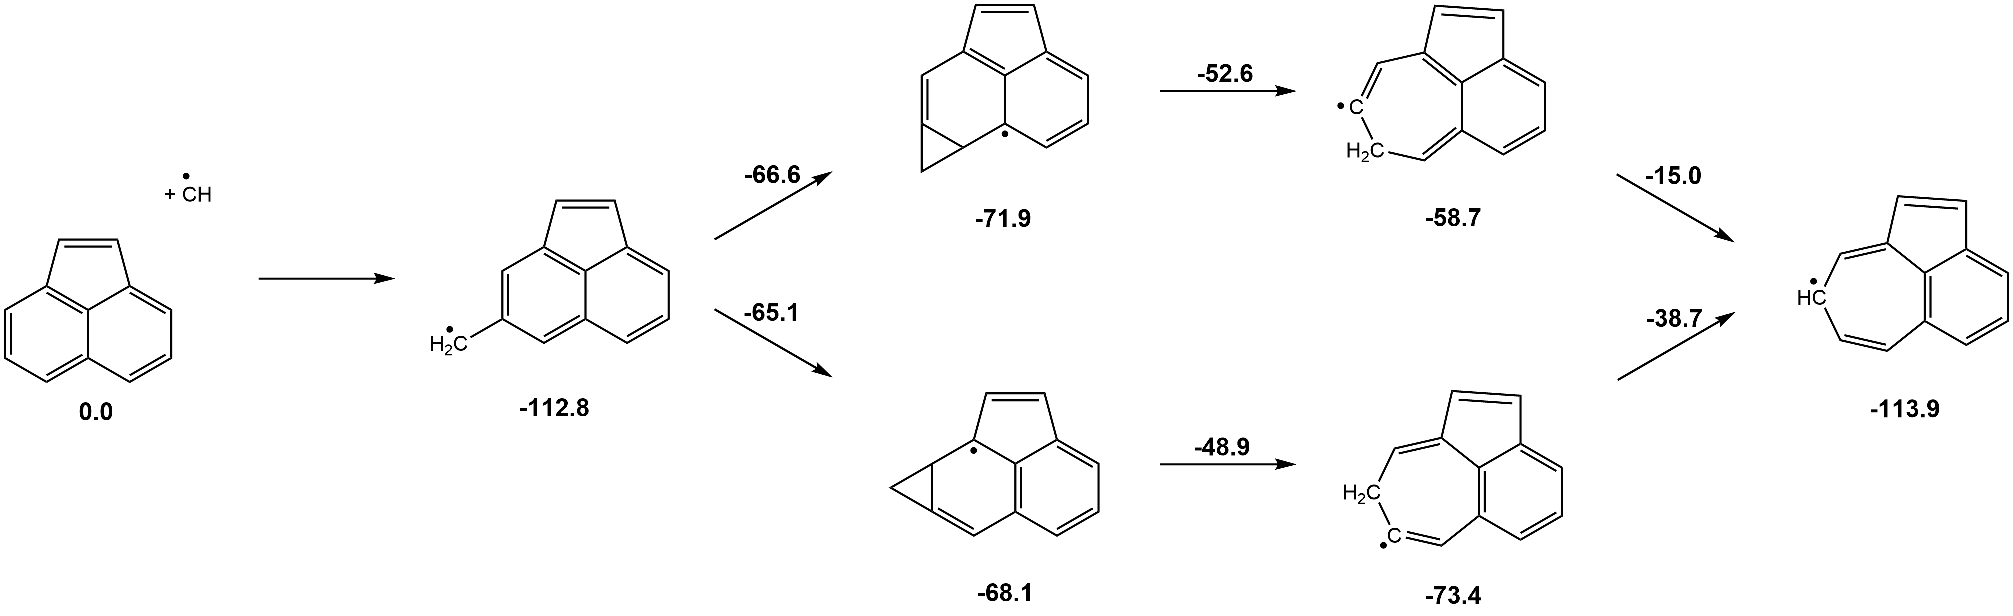
\includegraphics[width=1\textwidth]{Figures/FigS1}
	\caption{Reaction scheme for CH insertion at the 2-position, forming the second tropyl-like RSR. Calculations were performed at MO6-2X/6-31G(2df,p) level of theory. The energies are in kcal/mol.}
	\label{figS1}
\end{figure}

\begin{figure}[h!]
	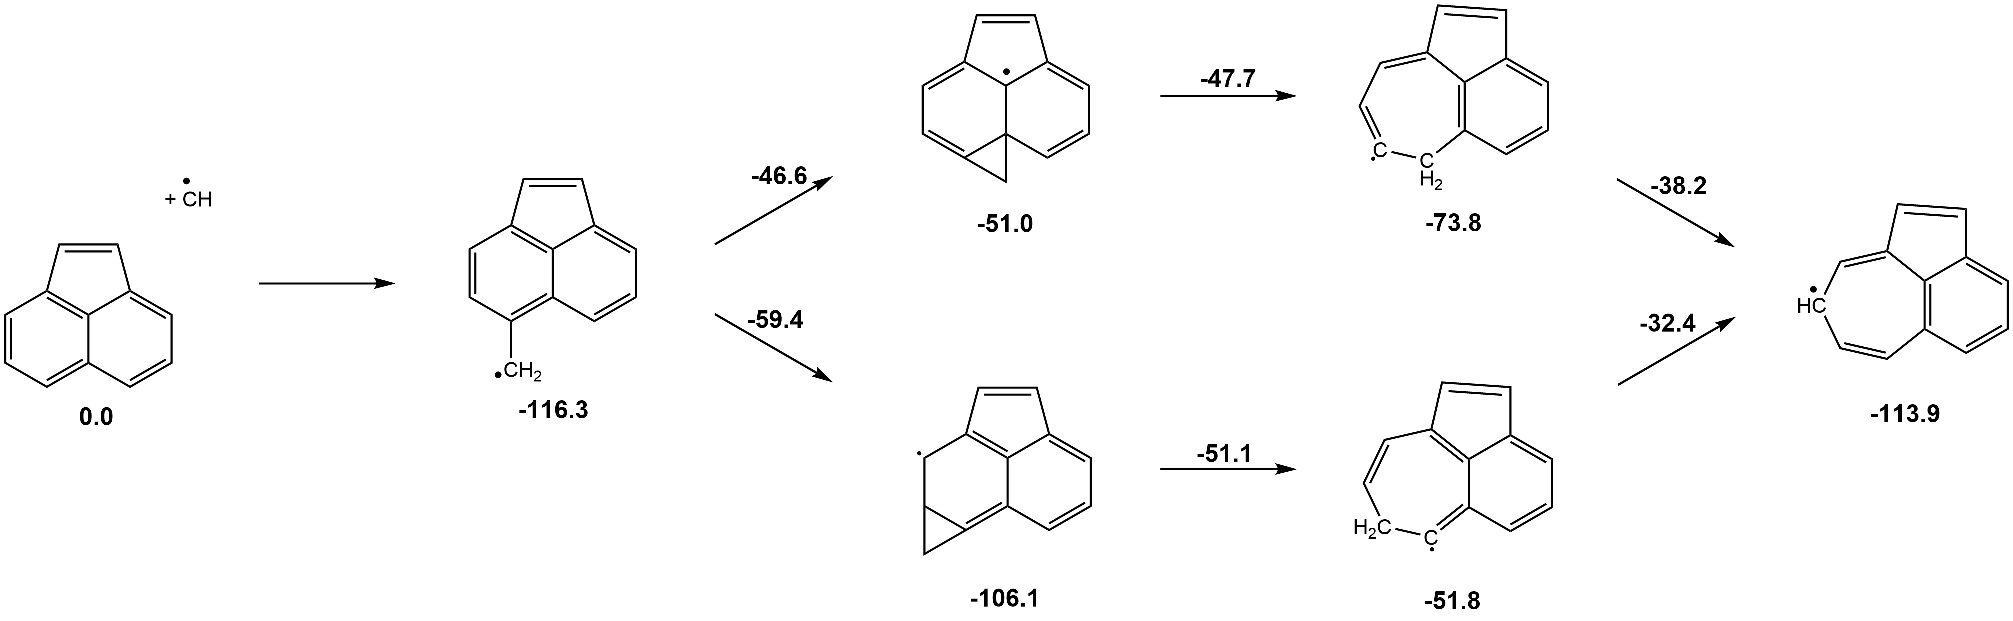
\includegraphics[width=1\textwidth]{Figures/FigS2}
	\caption{Reaction scheme for CH insertion at the 3-position, forming the third tropyl-like RSR. Calculations were performed at MO6-2X/6-31G(2df,p) level of theory. The energies are in kcal/mol.}
	\label{figS2}
\end{figure}


\end{document}